\title{Warm-Up for March 30th, 2022}
\author{Dr. Jordan Hanson - Whittier College Dept. of Physics and Astronomy}
\date{\today}
\documentclass[12pt]{article}
\usepackage[a4paper, total={18cm, 27cm}]{geometry}
\usepackage{graphicx}
\usepackage{amsmath}
\usepackage{bm}
\def\rcurs{{\mbox{$\resizebox{.16in}{.08in}{
\includegraphics{ScriptR}}$}}}
\def\brcurs{{\mbox{$\resizebox{.16in}{.08in}{
\includegraphics{BoldR}}$}}}
\def\hrcurs{{\mbox{$\hat \brcurs$}}}
 
\begin{document}
\maketitle
\small
\section{Memory Bank}
\begin{enumerate}
\item Bound surface charge: $\sigma_b = \mathbf{P} \cdot \hat{\mathbf{n}}$
\item Bound charge density: $\rho_b = -\nabla \cdot \mathbf{P}$
\item Potential \textit{inside} a sphere with radius $R$ and $\sigma(\theta) = k P_1(\cos\theta)$ on the surface:
\begin{equation}
V(r,\theta) = \frac{k}{3\epsilon_0}r\cos\theta \label{eq:2}
\end{equation}
\item Potential \textit{outside} a sphere with radius $R$ and $\sigma(\theta) = k P_1(\cos\theta)$ on the surface:
\begin{equation}
V(r,\theta) = \frac{kR^3}{3\epsilon_0 r^2}\cos\theta \label{eq:3}
\end{equation}
\end{enumerate}

\section{Bound Charge and Potential}

\begin{enumerate}
\item Find the potential and electric field produced by a uniformly polarized sphere of radius $R$.  (a) Note that $\mathbf{P} = P \hat{\mathbf{z}}$, and $\hat{\mathbf{n}} = \hat{\mathbf{r}}$.  What are $\rho_b$ and $\sigma_b$? (b) Use your knowledge of $\sigma_b$ and Eqs. \ref{eq:2} and \ref{eq:3} to determine $V(\mathbf{r})$ inside and outside the polarized sphere. (c) \textbf{Bonus:} what is $\mathbf{E}$ inside and outside?
\end{enumerate}

\begin{figure}
\centering
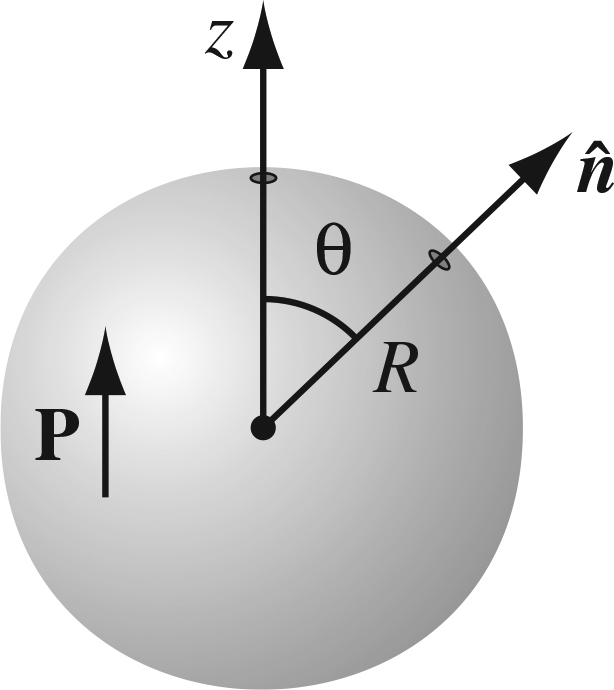
\includegraphics[width=0.2\textwidth]{figures/4_9.jpeg}
\caption{\label{fig:1} A uniformly polarized sphere.}
\end{figure}

\end{document}